\section{The impact of ignoring the S-wave in an angular analysis of \BdToKstll}
\label{sec:swave:ignore}

The effect of ignoring or including a \kpi S-wave was tested as a function of dataset 
 size in order to find a minimum dataset at which the bias 
 from ignoring the S-wave contribution to the angular distribution when measuring the angular observables becomes significant.
Datasets were generated for sample sizes ranging from 50 to 
1000 events and analysed assuming a pure P-wave state. 
The results are shown in Fig.~\ref{fig:bias}. 
\begin{figure}[tb]
\centering
\subfigure[]{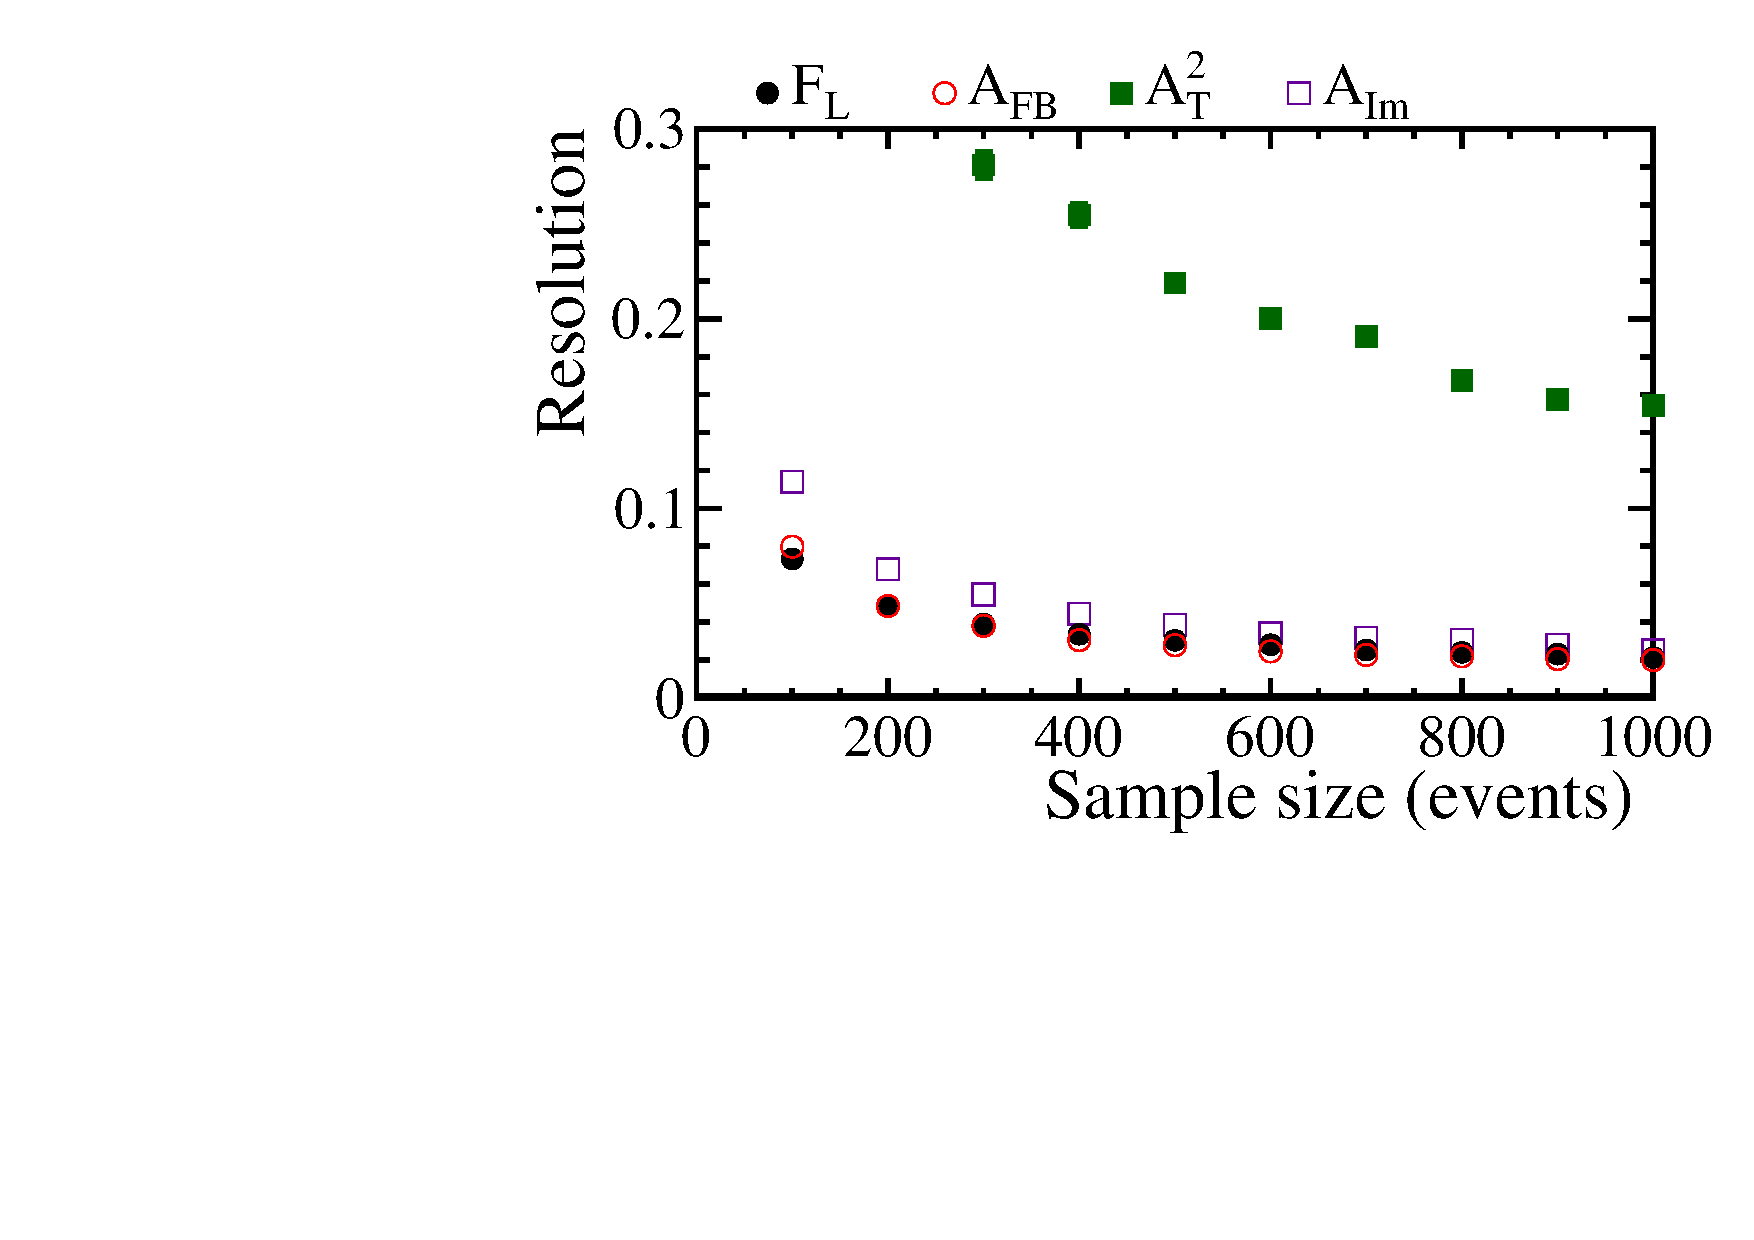
\includegraphics[width=0.48\textwidth]{chapter6/figs/fit_result_ds_gen_res.pdf}}
\subfigure[]{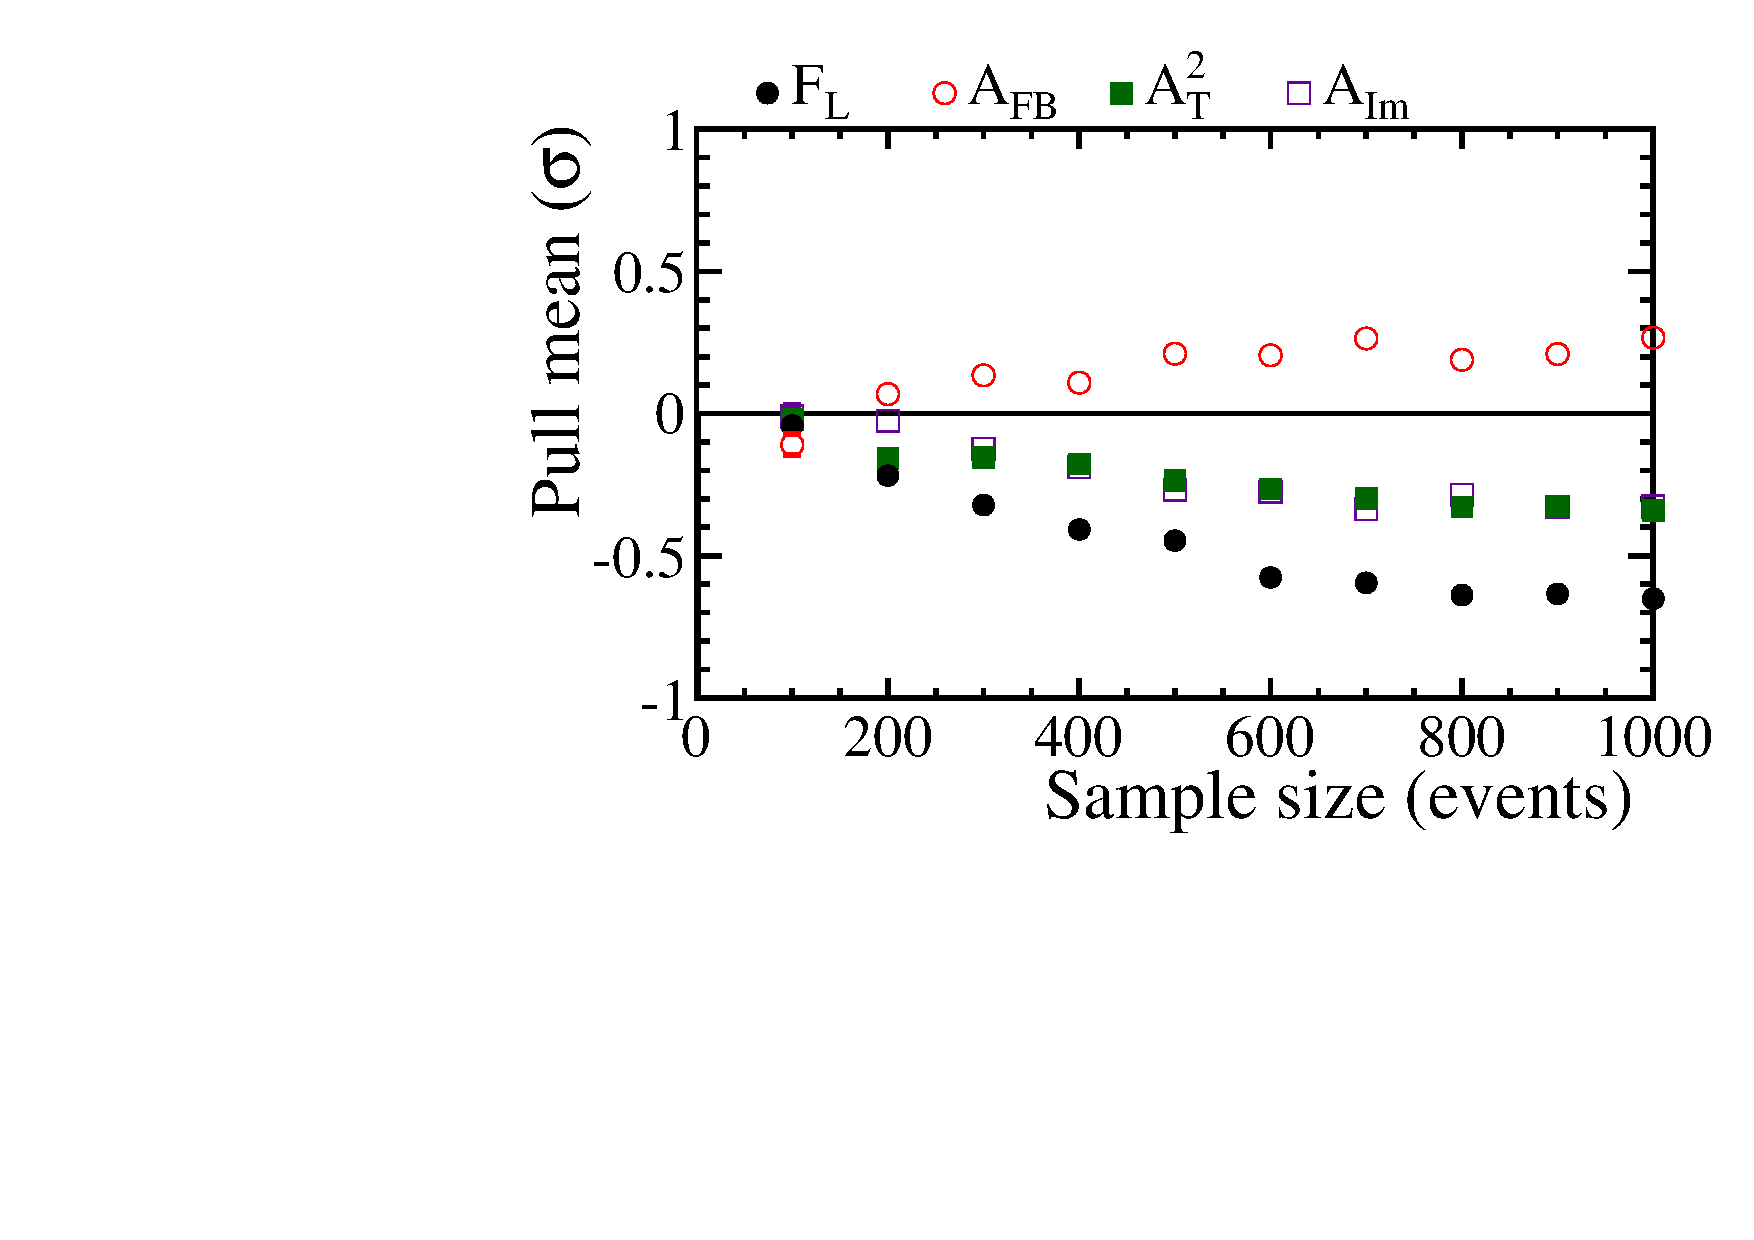
\includegraphics[width=0.48\textwidth]{chapter6/figs/fit_result_ds_gen_mean.pdf}}
\subfigure[]{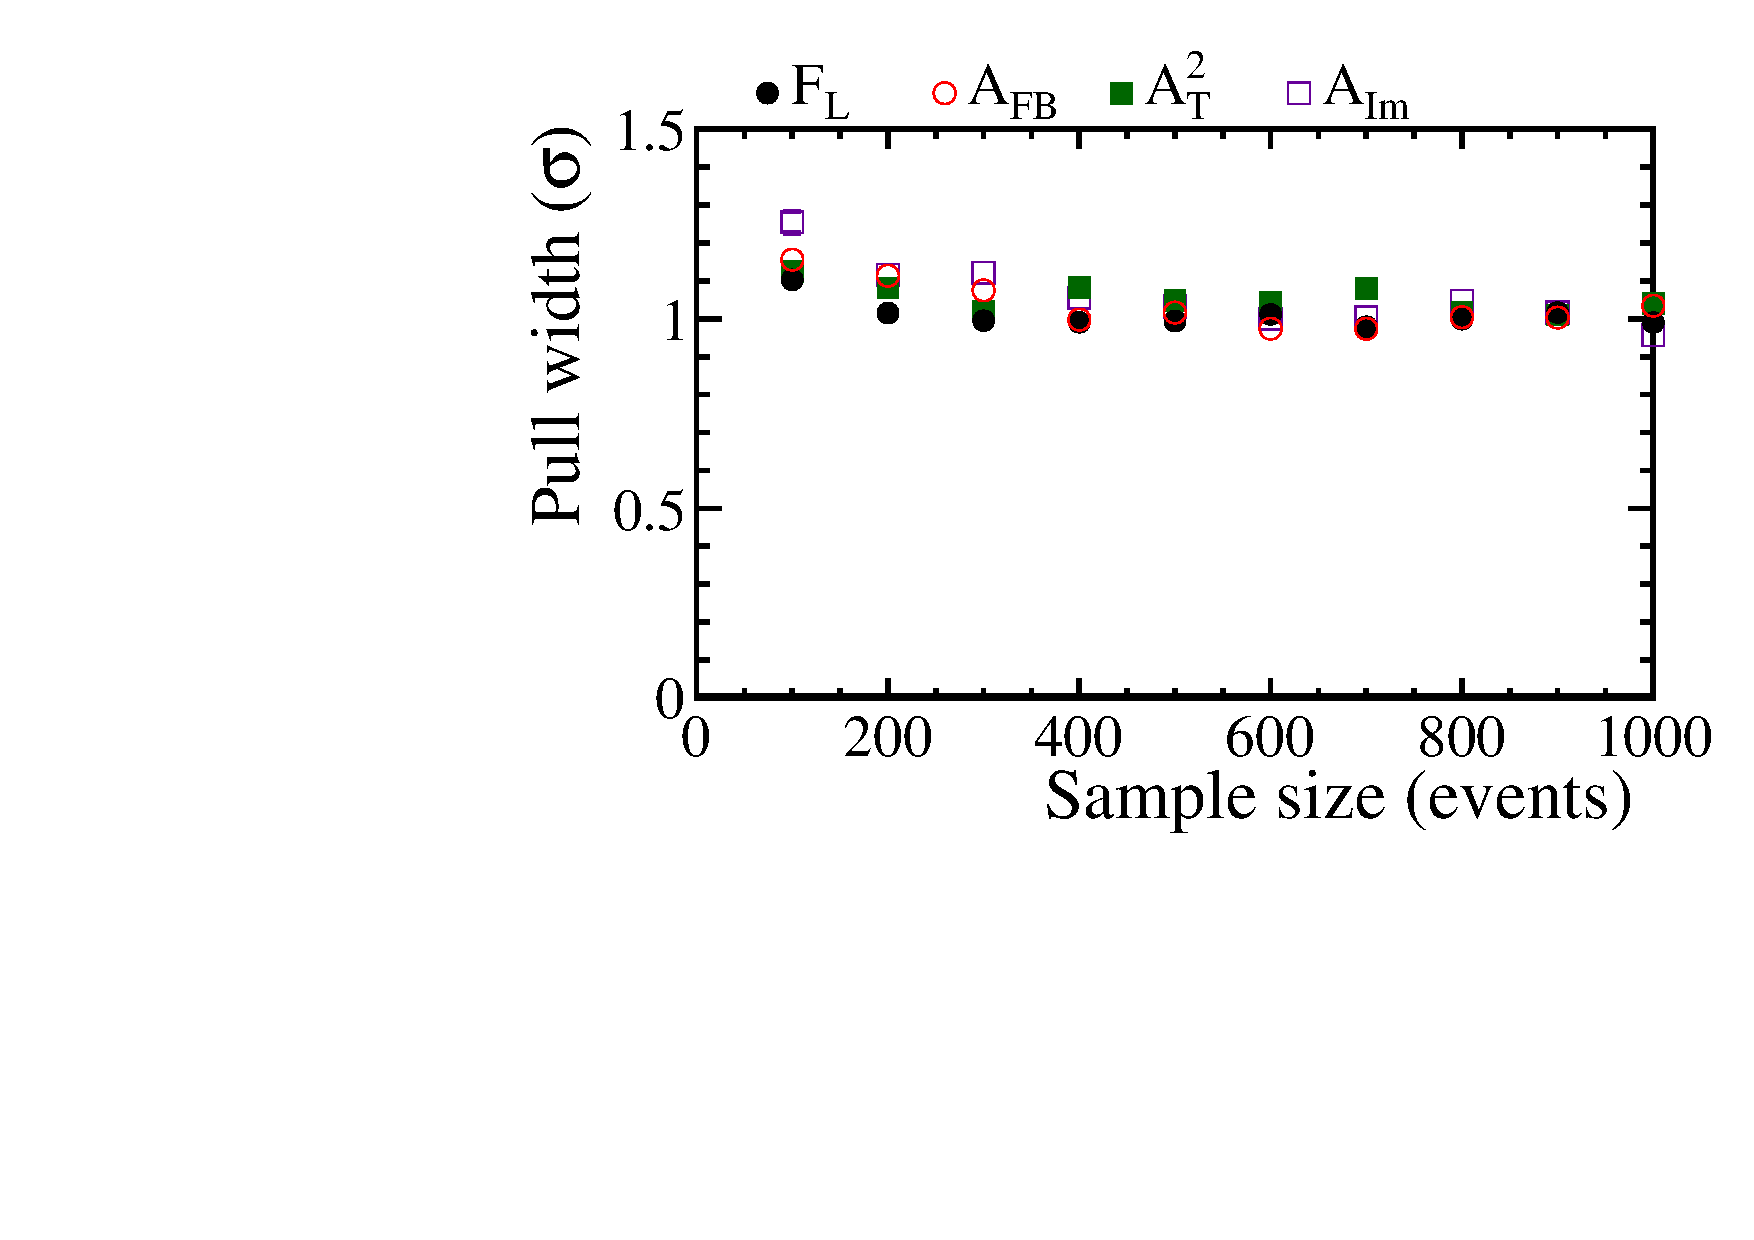
\includegraphics[width=0.48\textwidth]{chapter6/figs/fit_result_ds_gen_width.pdf}}
\caption[ Resolution, pull mean and width of 
1000 toy datasets analysed as a pure P-wave state as a 
function of dataset size.    ]
{Resolution (a), pull mean (b) and pull width (c) of 
1000 toy datasets analysed as a pure P-wave state as a 
function of dataset size. It can be seen that the bias 
on the observable (non-zero pull mean) increases dramatically as the sample 
size increases. This is because the statistical error 
decreases increasing the sensitivity to the ignored S-wave 
contribution. The bias of \AFB is positive  
because \AFB is negative in the \qsq bin chosen. 
~\label{fig:bias}}
\end{figure}

From Eq.~\ref{eq:theo4d}, it can be seen that \AT2 
has a factor of (1-\FL) in front of it. The large 
value of \FL used to generated datasets is 
in turn causing \AT2 to have a much worse 
resolution than \AFB, \FL and \OS3 . There is 
significant bias (non-zero mean) of the pull distribution for all
 observables when the S-wave is ignored in the angular distribution for datasets 
 of more than 200 events. This corresponds to a 
 change of 0.2$\sigma$ in \FL for a dataset of 200 events.
The behaviour can be understood in terms of the $(1-\FS)$ 
factor in Eq.~\ref{eq:theo4d}. It gives an offset to the 
fitted values of the observables which are proportional 
to the value of $(1-\FS)$.

The angular fit was performed on toy 
datasets with an increasing S-wave contribution.
Datasets of 500 events were generated with a 
varying S-wave contribution in the narrow \psq
 mass window of ($800 < p < 1000 \mev$) 
 from no S-wave up to a \FS value of $0.4$. 
The resolution and the mean and width of the pull 
distribution for each of the four observables
 (\AFB, \FL, \AT2 , \OS3 ) were calculated and 
 the results are shown in Fig.~\ref{fig:fsval}.
\begin{figure}[tb]
\centering
\subfigure[]{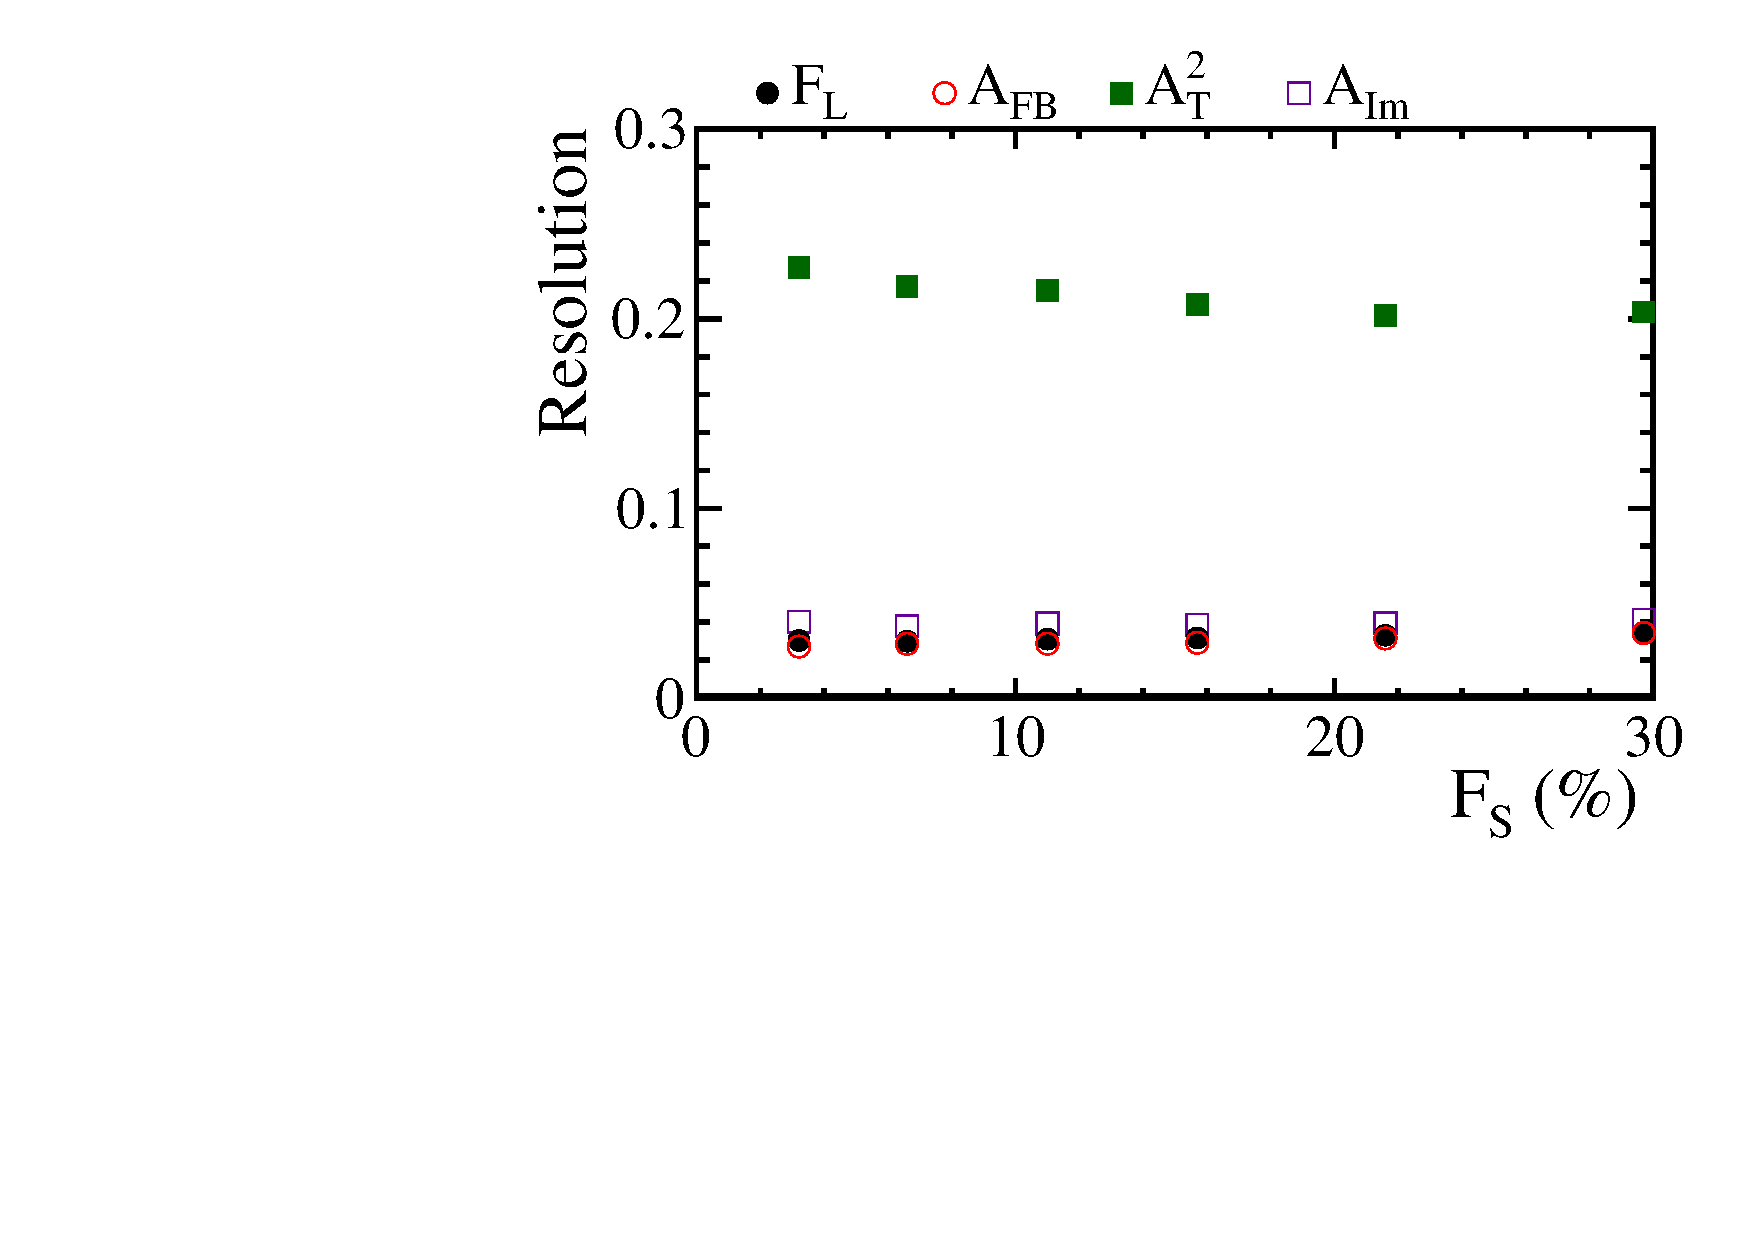
\includegraphics[width=0.48\textwidth]{chapter6/figs/fit_result_fs_gen_res.pdf}}
\subfigure[]{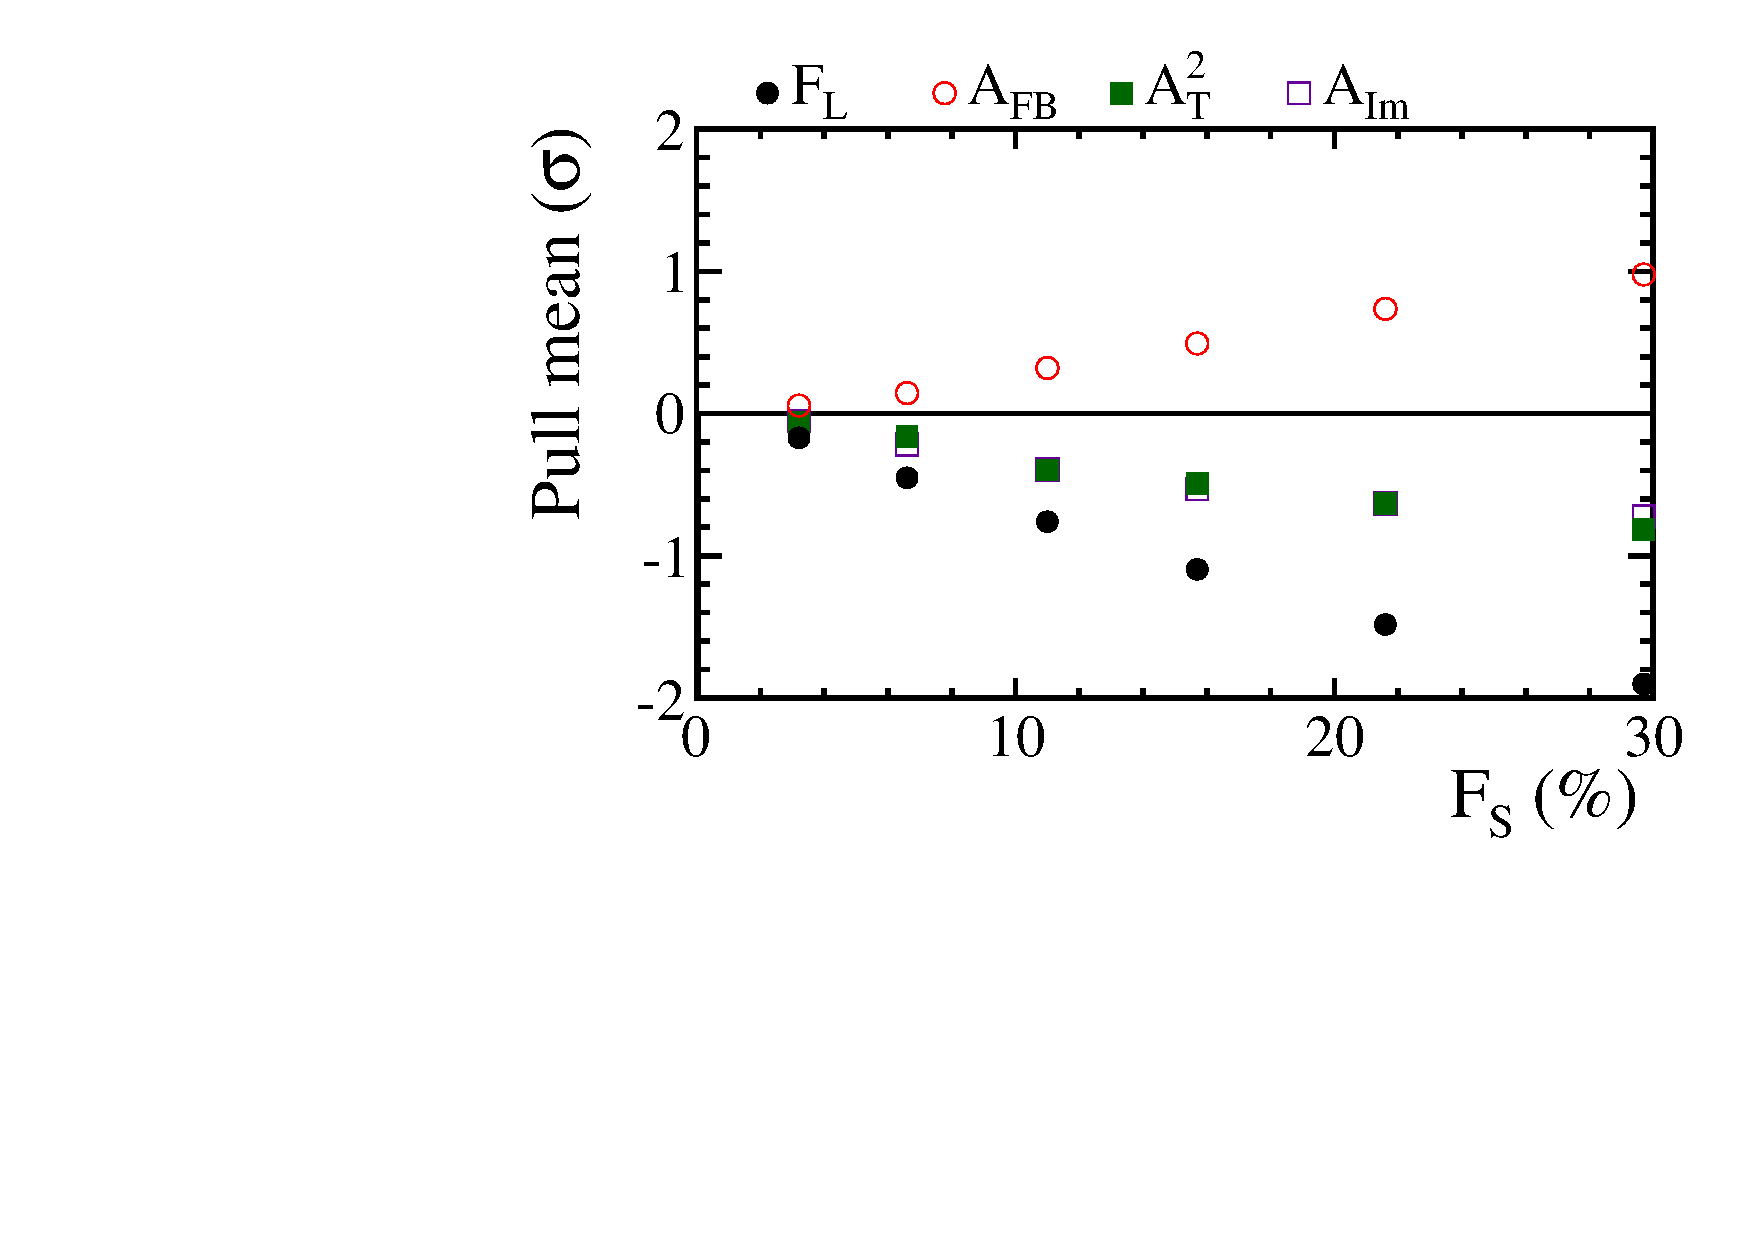
\includegraphics[width=0.48\textwidth]{chapter6/figs/fit_result_fs_gen_mean.pdf}}
\subfigure[]{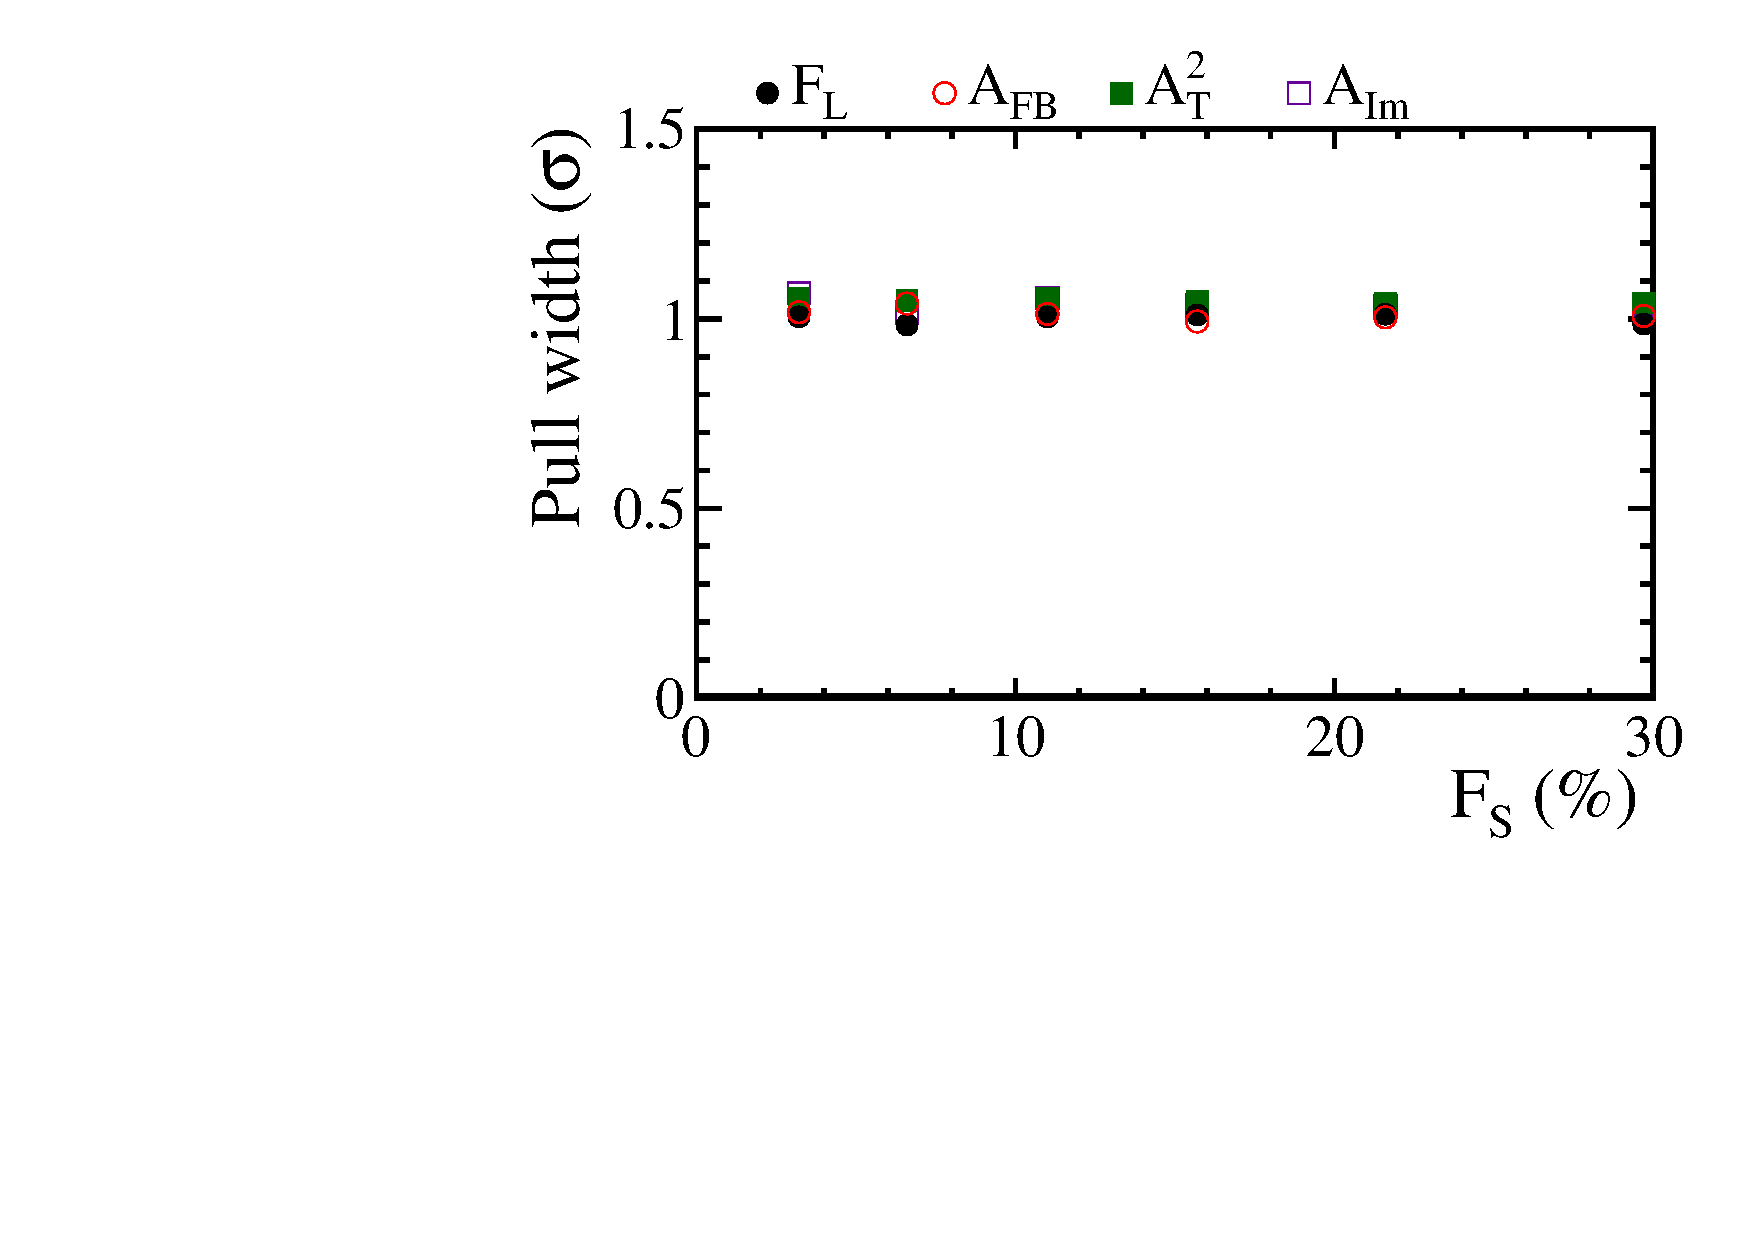
\includegraphics[width=0.48\textwidth]{chapter6/figs/fit_result_fs_gen_width.pdf}}
\caption[ The resolution, mean and width of the pull distribution 
of 1000 toy datasets analysed as a pure 
P-wave state as a function of the S-wave contribution.   ]
{The resolution (a) the mean (b) and the width (c) of the pull distribution
of 1000 toy datasets analysed as a pure 
P-wave state as a function of S-wave contribution. 
The resolution and the bias can be seen to increase with the size of the S-wave 
contribution in a linear fashion. ~\label{fig:fsval}}
\end{figure}
Significant bias is seen in the angular 
observables when the S-wave is ignored for an S-wave magnitude of greater than 5\%.
The linear increase in the bias 
is another consequence of the (1-\FS) factor in the angular distribution.

